\section{Desenvolvimento do código}

O código foi desenvolvido utilizando o Visual Studio Code (VSCode) e a extensão do PlatformIO. Na página inicial, criamos o projeto com nome "wifi\_manager\_", utilizando a placa Espressif ESP32 Dev Module e o framework Arduino.

\subsection{Instalação das bibliotecas}

Para a realização do projeto, foi necessário a uso de duas biblioteca: AsynTCP e ESPAsyncWebServer. As duas bibliotecas podem ser adicionadas ao projeto pela seção de livrarias do PlatformIO, mas não foi necessário.

No arquivo \textit{platformio.ini}, colocamos o seguinte código para que todas as dependências para a realização do projeto sejam adicionadas, sem necessitar instalar as bibliotecas.

\begin{lstlisting}
lib_deps = ESP Async WebServer
\end{lstlisting}

Também é necessário para a realização do projeto utilizar o gerenciador de arquivos LittleFS, então no mesmo arquivo \textit{platformio.ini}, escrevemos o seguinte código:

\begin{lstlisting}
board_build.filesystem = littlefs
\end{lstlisting}

Por último, definimos a taxa de atualização do monitor para 9600.

\begin{lstlisting}
monitor_speed = 9600
\end{lstlisting}



\subsection{Escrevendo HTML das páginas WEB}

As páginas são bem simples. Há uma página \textit{index} e uma página de formulário para passar as credenciais da rede. As páginas e o arquivo de estilização precisam estar numa pasta chamada \textit{data} para serem enviadas ao ESP32.

A página \textit{index} só mostra se o botão selecionado é ON ou OFF. É uma página padrão para o fim do projeto.

\begin{lstlisting}
<div class="content">
  <div class="card-grid">
    <div class="card">
      <p class="card-title"><i class="fas fa-lightbulb"></i> GPIO 2</p>
      <p>
        <a href="on"><button class="button-on">ON</button></a>
        <a href="off"><button class="button-off">OFF</button></a>
      </p>
      <p class="state">State: %STATE%</p>
    </div>
  </div>
</div>
\end{lstlisting}

A página \textit{wifimanager} possui um formulário para passar as credenciais da rede e definir um endereço de acesso ao ESP32 que estará em modo estacionário.

\begin{lstlisting}
<form action="/" method="POST">
  <p>
    <label for="ssid">SSID</label>
    <input type="text" id ="ssid" name="ssid"><br>
    <label for="pass">Password</label>
    <input type="text" id ="pass" name="pass"><br>
    <label for="ip">IP Address</label>
    <input type="text" id ="ip" name="ip" value="192.168.1.200"><br>
    <label for="gateway">Gateway Address</label>
    <input type="text" id ="gateway" name="gateway" value="192.168.1.1"><br>
    <input type ="submit" value ="Submit">
  </p>
</form>
\end{lstlisting}

O código apresentado é apenas uma parte. Para acessá-lo por completo, assim como o arquivo \textit{css} para estilização, acesse os arquivos por esse \href{https://github.com/fabricio-araujo94/microcontroladores/tree/main/wifi_manager_/data}{repositório}.

Para enviar esses arquivos ao ESP32, acessamos a página do PlatformIO, expandimos o menu com o nome da placa com a qual estamos desenvolvendo o projeto (o nosso caso se chama \textit{esp32dev}) e expandimos o menu Platform. Para assim, clicarmos em \textit{Build Filesystem Image}, e quando acabar, clicamos em \textit{Upload Filesystem Image} para enviar os arquivos.

\begin{figure}[H]
    \centering
    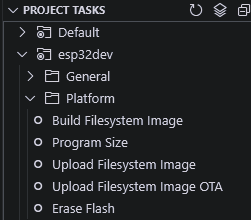
\includegraphics[width=0.5\linewidth]{img/build_image.png}
    \caption{Criando imagem.}
    \label{fig:build-image}
\end{figure}

\subsection{}

Para começar, importamos todas as bibliotecas necessárias.

\begin{lstlisting}
#include "LittleFS.h"
#include <Arduino.h>
#include <AsyncTCP.h>
#include <ESPAsyncWebServer.h>
#include <WiFi.h>
\end{lstlisting}

Então, criamos um objeto da classe AsyncWebServer.

\begin{lstlisting}
AsyncWebServer server(80);
\end{lstlisting}

Criamos constantes para guardar o nome dos parâmetro, assim como o endereço dos arquivos de cada parâmetro. Também criamos variáveis para guardar as informações.

\begin{lstlisting}
#define PARAM_INPUT_1 "ssid"
#define PARAM_INPUT_2 "pass"
#define PARAM_INPUT_3 "ip"
#define PARAM_INPUT_4 "gateway"

String ssid;
String pass;
String ip;
String gateway;

const char *ssidPath = "/ssid.txt";
const char *passPath = "/pass.txt";
const char *ipPath = "/ip.txt";
const char *gatewayPath = "/gateway.txt";
\end{lstlisting}

Instaciamos dois objetos da classe IPAddress. Um para o endereço IP do ESP32 e outro para o endereço IP do gateway. Também definimos a máscara da rede.

\begin{lstlisting}
IPAddress localIP;
IPAddress localGateway;
IPAddress subnet(255, 255, 0, 0);
\end{lstlisting}

Também criamos variáveis para calcular o tempo de tentativa de conexão com a rede Wi-Fi.

\begin{lstlisting}
unsigned long previousMillis = 0;
int interval = 10000;
\end{lstlisting}

A função \textit{initLittleFS} inicializa o gerenciador de arquivos com a função \textit{begin}.

\begin{lstlisting}
void initLittleFS() {
  if (!LittleFS.begin(true)) {
    Serial.println("An error has occurred while mounting LittleFS");
  }
  Serial.println("LittleFS mounted successfully");
}
\end{lstlisting}

A função \textit{readFile} lê e retorna o conteúdo do arquivo do caminho especificado.

\begin{lstlisting}
String readFile(fs::FS &fs, const char *path) {
  Serial.printf("Reading file: %s\r\n", path);

  File file = fs.open(path);
  if (!file || file.isDirectory()) {
    Serial.println("- failed to open file for reading");
    return String();
  }

  String fileContent;
  while (file.available()) {
    fileContent = file.readStringUntil('\n');
    break;
  }
  return fileContent;
}
\end{lstlisting}

Na função \textit{writeFile}, escrevemos a mensagem no arquivo de um caminho especificado.

\begin{lstlisting}
void writeFile(fs::FS &fs, const char *path, const char *message) {
  Serial.printf("Writing file: %s\r\n", path);

  File file = fs.open(path, FILE_WRITE);
  if (!file) {
    Serial.println("- failed to open file for writing");
    return;
  }
  if (file.print(message)) {
    Serial.println("- file written");
  } else {
    Serial.println("- write failed");
  }
}
\end{lstlisting}

A função \textit{initWifi} tenta se conectar à uma rede Wi-Fi e retorna um booleano se ele foi bem sucedido ou não.

\begin{lstlisting}
bool initWiFi() {
...
\end{lstlisting}

No começo, ela configura o módulo Wi-fi em modo estacionário e define o endereço IP do dispositivo e do gateway.

\begin{lstlisting}
WiFi.mode(WIFI_STA);
localIP.fromString(ip.c_str());
localGateway.fromString(gateway.c_str());

if (!WiFi.config(localIP, localGateway, subnet)) {
    Serial.println("STA Failed to configure");
    return false;
}
\end{lstlisting}

Logo após, a tentativa de conexão é feita utilizando o método \textit{begin}.

\begin{lstlisting}
WiFi.begin(ssid.c_str(), pass.c_str());
\end{lstlisting}

Agora, é o momento de espera para conferir se a conexão foi realizada. Caso exceda o tempo limite, a função retorna falso. É importante que não se espere para sempre, pois isso implica que a conexão não foi realizada e é necessário tentar entrar em outra rede.

\begin{lstlisting}
unsigned long currentMillis = millis();
previousMillis = currentMillis;

while (WiFi.status() != WL_CONNECTED) {
    currentMillis = millis();
    
    // evita que o ESP tente conectar a rede muitas vezes
    if (currentMillis - previousMillis >= interval) {
      Serial.println("Failed to connect.");
      return false;
    }
}
\end{lstlisting}

Se tudo ocorreu bem, a função retorna verdadeiro.



\subsection{Função setup}

Inicializamos o \textit{Serial} com a taxa de 9600.

\begin{lstlisting}
void setup() {
    Serial.begin(9600);
\end{lstlisting}

Inicializamos o Little FS, lemos os arquivos que estão salvos no ESP32 e salvamos nas variáveis.

\begin{lstlisting}
initLittleFS();

ssid = readFile(LittleFS, ssidPath);
pass = readFile(LittleFS, passPath);
ip = readFile(LittleFS, ipPath);
gateway = readFile(LittleFS, gatewayPath);

Serial.println(ssid);
Serial.println(pass);
Serial.println(ip);
Serial.println(gateway);
\end{lstlisting}

A exibição das páginas funcionam dessa maneira: se o ESP32 estiver conectado a um rede, é exibido a página \textit{index}; e se não estiver, é exibido a página do Wi-Fi Manager.

Para a exibição de cada página, precisamos utilizar o método \textit{serverStatic} para dizer que os arquivos de um certo diretório são arquivos estáticos. Salvamos os arquivos HTML e CSS na raiz do gerenciador de arquivos, e a pasta raiz se chama "LittleFS".

\begin{lstlisting}
server.serveStatic("/", LittleFS, "/");
\end{lstlisting}

Essa é a implementação para quando a conexão estiver feita.

\begin{lstlisting}
if (initWiFi()) {
    // envia a pagina index
    server.on("/", HTTP_GET, [](AsyncWebServerRequest *request) {
      request->send(LittleFS, "/index.html", "text/html");
    });
    server.serveStatic("/", LittleFS, "/");
    
    server.begin();
\end{lstlisting}

O caso da conexão não ter sido feita é mais trabalhosa, pois precisamos que o ESP32 se torne um \textit{access point} para que outro dispositivo possa se conectar a ele. Isso é possível utilizando o método \textit{SOFTAP} do módulo WiFi, onde definimos o SSID e uma senha. No nosso projeto, utilizamos NULL para que não seja necessário utilizar uma senha.

Também precisamos informar ao usuário qual o endereço IP que ele deve acessar para entrar na página do Wifi Manager. Conseguimos o IP com o meétodo \textit{softAPIP} e imprimimos no monitor.

\begin{lstlisting}
Serial.println("Setting AP (Access Point)");
WiFi.softAP("ESP-WIFI-MANAGER", NULL);

IPAddress IP = WiFi.softAPIP();
Serial.print("AP IP address: ");
Serial.println(IP);
\end{lstlisting}

Enviamos a página HTML \textit{WIFIMANAGER}.

\begin{lstlisting}
server.on("/", HTTP_GET, [](AsyncWebServerRequest *request) {
    request->send(LittleFS, "/wifimanager.html", "text/html");
});
server.serveStatic("/", LittleFS, "/");
\end{lstlisting}

No código HTML, quando o usuário apertar o botão de \textit{submit}, os dados irão para a mesma URL só que com o método POST, e é nessa parte que pegamos os dados e escrevemos em arquivos no ESP32.

Com o método \textit{params}, conseguimos a quantidade de parâmetros que foram enviados.

\begin{lstlisting}
server.on("/", HTTP_POST, [](AsyncWebServerRequest *request) {
  int params = request->params();
\end{lstlisting}

Utilizamos um laço \textit{for} para pegar todos os parâmetros e escrever em um arquivo. Conseguimos resgatar os parâmetros utilizando o método \textit{getParam} e passando a sua posição. Ele retorna um ponteiro da classe AsyncWebParameter. Utilize o método \textit{isPost} para conferir se o parâmetro é do tipo POST.

\begin{lstlisting}
for (int i = 0; i < params; i++) {
    const AsyncWebParameter *p = request->getParam(i);
    if (p->isPost()) {
\end{lstlisting}

Precisamos conferir qual é o nome do parâmetro comparando com as quatro opções de parâmetros que existem. Em seguida, copiamos seu conteúdo para sua variável correspondente e utilizamos a função \textit{writeFile} para escrever o parâmetro num arquivo. Esse processo se repete com cada parâmetro

\begin{lstlisting}
// ssid
if (p->name() == PARAM_INPUT_1) {
    ssid = p->value().c_str();
    Serial.print("SSID set to: ");
    Serial.println(ssid);
    writeFile(LittleFS, ssidPath, ssid.c_str());
}
\end{lstlisting}

Um adendo que essa variável a qual o conteúdo é copiado é a variável global que foi criada no começo do código. É necessário para a conexão Wi-Fi que será realizada.

Feito tudo isso, informamos que o processo e reiniciamos o ESP32.

\begin{lstlisting}
request->send(200, "text/plain",
                "Done. ESP will restart, connect to your router and go to "
                "IP address: " +
                ip);
delay(3000);
ESP.restart();
\end{lstlisting}

Por fim, iniciamos o server.

\begin{lstlisting}
server.begin();
\end{lstlisting}